\documentclass{article}

% Add 'authorblk' package for affliation support
\usepackage{authblk}

% use package to control paper dimensions
\usepackage{geometry}
 \geometry{
		a4paper,
		left=22mm,
		right=22mm,
		top=20mm,
		bottom=20mm
	}
	
\usepackage{graphicx}
\usepackage{subcaption}


% use packages for code listings
\usepackage{listings}
\usepackage{color}

\definecolor{mGreen}{rgb}{0,0.6,0}
\definecolor{mGray}{rgb}{0.5,0.5,0.5}
\definecolor{mPurple}{rgb}{0.58,0,0.82}
\definecolor{backgroundColour}{rgb}{0.95,0.95,0.92}

\lstdefinestyle{CStyle}{
    backgroundcolor=\color{backgroundColour},   
    commentstyle=\color{mGreen},
    keywordstyle=\color{magenta},
    numberstyle=\tiny\color{mGray},
    stringstyle=\color{mPurple},
    basicstyle=\footnotesize,
    breakatwhitespace=false,         
    breaklines=true,                 
    captionpos=b,                    
    keepspaces=true,                 
    showspaces=false,                
    showstringspaces=false,
    showtabs=false,                  
    tabsize=2,
    language=C
}

\usepackage{multirow}

\title{Analyzing Performance of Spatial-Domain Linear Filtering on Multi-Channel Images using OpenMP}
\author{R Mukesh}
\affil{IIITDM, Kancheepuram}

\date{September 3, 2018}

\begin{document}
	\maketitle
	
	\begin{abstract}
		Typically, Image Processing Algorithms are massively parallelizable and are performed on specialized hardwares such as Graphics Processing units(GPUs) that offer high-throughput. This experiment aims to analyze the performance of parallelized Spatial-Domain linear filtering for multi-channel images using OpenMP.
	\end{abstract}
	
	\section{Theory}
	
		\subsection{Spatial-Domain Linear Filtering}
			\textbf{Linear Filtering} is neighborhood operation, in the which the value of any given pixel in the output image is represented as a linear function of the pixel values in the neighborhood of the corresponding input pixel. Linear filtering in spatial domain is performed using \textbf{convolution}.
			
			\textbf{Mean Filtering} is a linear filtering in which value of any given pixel in the ouput image is the mean of values of pixel in a \(kxk\) window centered at the corresponding input pixel (where k is an odd number).
					
		\subsection{Sections in OpenMP}
			
			The section construct in OpenMP is a way of distributing different independent blocks of codes (each performing a task) to different threads. The sytax of the sections construct is:
			
		\begin{lstlisting}[style=CStyle]
		
			#pragma omp parallel
			{
				#pragma omp sections
				{
					#pragma omp section
					{
						//structured block 1
					}
					
					#pragma omp section
					{
						//structured block 2
					}
					
					#pragma omp section
					{
						//structured block 3
					}
					
					...
				}
			}
		\end{lstlisting}				
			
	\section{Results \protect\footnote{The experiments were conducted on a computer with 6\textsuperscript{th} Generation Intel(R) Core(TM) i7-6500U Processor (4M Cache, upto 3.10 GHz) and 4GB Single Channel DDR3L 1600M Hz (4GBx1) RAM.}}
	
		The experiments were conducted on a three-channel (red, green and blue) image of size 384x512 for varying size of filter kernels. Each section block performed mean filtering of one channel of the image.

	
\begin{table}[!htbp]
\begin{tabular}{|c|c|c|c|c|c|c|}
\hline
\multicolumn{1}{|l|}{\multirow{3}{*}{\textbf{Number of Threads}}} & \multicolumn{6}{c|}{\textbf{Execution Time (in seconds)}}                                                                         \\ \cline{2-7} 
\multicolumn{1}{|l|}{}                                            & \multicolumn{3}{c|}{\textbf{Without Sections}}                  & \multicolumn{3}{c|}{\textbf{With Sections}}                     \\ \cline{2-7} 
\multicolumn{1}{|l|}{}                                            & \textbf{3x3 filter} & \textbf{5x5 filter} & \textbf{7x7 filter} & \textbf{3x3 filter} & \textbf{5x5 filter} & \textbf{7x7 filter} \\ \hline
1                                                                 & 0.019927            & 0.054407            & 0.105519            & 0.012785            & 0.021406            & 0.040657            \\ \hline
2                                                                 & 0.010053            & 0.027356            & 0.053044            & 0.008516            & 0.021233            & 0.040614            \\ \hline
4                                                                 & 0.007793            & 0.015653            & 0.032042            & 0.009176            & 0.021220            & 0.040507            \\ \hline
6                                                                 & 0.007935            & 0.020113            & 0.038913            & 0.008530            & 0.021251            & 0.040530            \\ \hline
8                                                                 & 0.007302            & 0.015856            & 0.030059            & 0.008977            & 0.021224            & 0.040493            \\ \hline
12                                                                & 0.007650            & 0.016432            & 0.034132            & 0.008535            & 0.021301            & 0.040629            \\ \hline
16                                                                & 0.007699            & 0.017675            & 0.031378            & 0.008656            & 0.021210            & 0.040533            \\ \hline
20                                                                & 0.007568            & 0.019941            & 0.033236            & 0.008595            & 0.021234            & 0.040508            \\ \hline
24                                                                & 0.009263            & 0.020189            & 0.031605            & 0.008533            & 0.021246            & 0.040567            \\ \hline
28                                                                & 0.007752            & 0.025205            & 0.033459            & 0.008351            & 0.021210            & 0.043062            \\ \hline
32                                                                & 0.008162            & 0.022908            & 0.032675            & 0.010023            & 0.021207            & 0.043040            \\ \hline
\end{tabular}
\end{table}

\textbf{Note:} The actual number of concurrently executing threads for the programs with sections is thrice the indicated number since the three sections are executed in parallel, with each section executing the indicated number of threads.

\begin{figure}[!htbp]

	\centering
	\begin{subfigure}[!htbp]{\textwidth}
		\centering
		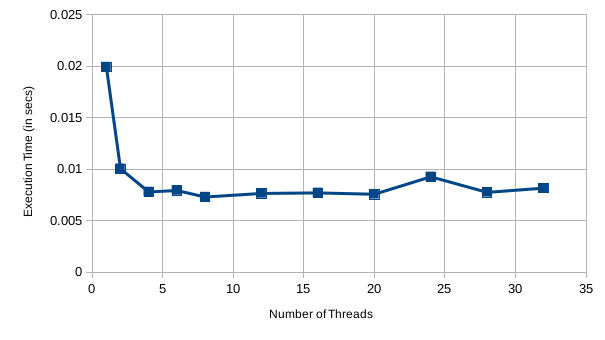
\includegraphics[scale=0.8]{without-sections-3x3-performance}
		\subcaption{Performance of Mean Filtering for 3x3 Filter (without sections)}
	\end{subfigure}
	
	\begin{subfigure}[!htbp]{\textwidth}
		\centering
		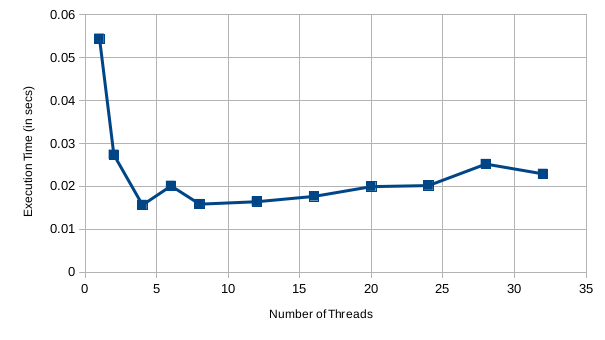
\includegraphics[scale=0.8]{without-sections-5x5-performance}
		\subcaption{Performance of Mean Filtering for 5x5 Filter (without sections)}
	\end{subfigure}
	
	\begin{subfigure}[!htbp]{\textwidth}
		\centering
		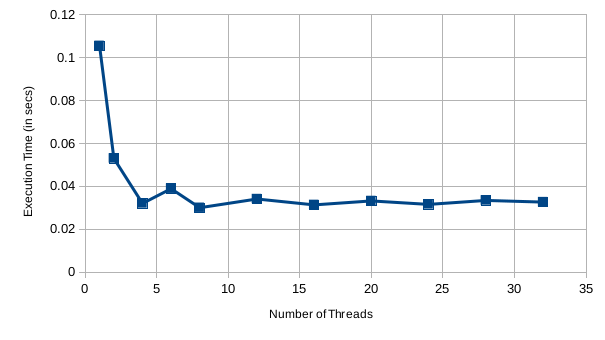
\includegraphics[scale=0.8]{without-sections-7x7-performance}
		\subcaption{Performance of Mean Filtering for 7x7 Filter (without sections)}
	\end{subfigure}
	
	\caption{Number of Threads vs Execution Time of Mean Filtering for varying filter size in OpenMP without sections}
\end{figure}

\begin{figure}[!htbp]

	\centering
	\begin{subfigure}[!htbp]{\textwidth}
		\centering
		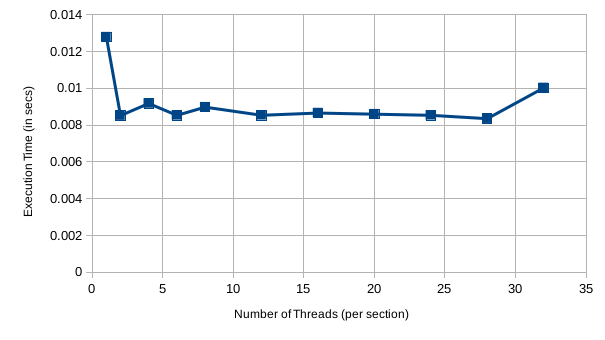
\includegraphics[scale=0.8]{with-sections-3x3-performance}
		\subcaption{Performance of Mean Filtering for 3x3 Filter (with sections)}
	\end{subfigure}
	
	\begin{subfigure}[!htbp]{\textwidth}
		\centering
		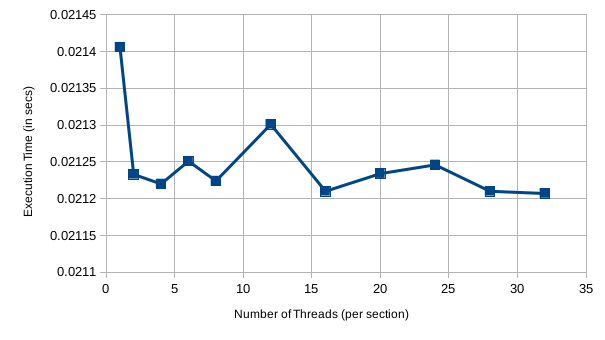
\includegraphics[scale=0.8]{with-sections-5x5-performance}
		\subcaption{Performance of Mean Filtering for 5x5 Filter (with sections)}
	\end{subfigure}
	
	\begin{subfigure}[!htbp]{\textwidth}
		\centering
		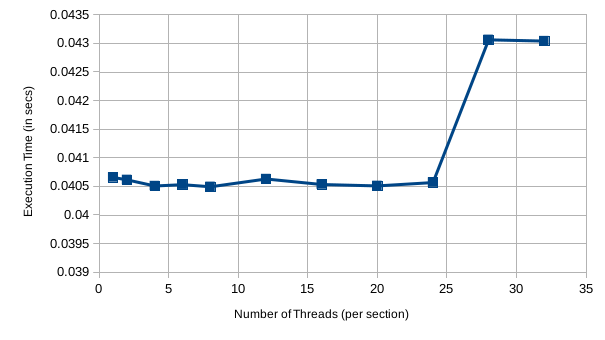
\includegraphics[scale=0.8]{with-sections-7x7-performance}
		\subcaption{Performance of Mean Filtering for 7x7 Filter (with sections)}
	\end{subfigure}
	
	\caption{Number of Threads vs Execution Time of Mean Filtering for varying filter size in OpenMP with sections}
\end{figure}

\section{Calculation}

The parallel fraction of the algorithm can be computed using the following equation:

\begin{equation}
	f = \frac{(1-T_p/T_1)}{(1-1/p)}
\end{equation}

For Mean Filtering using 3x3 filter (without sections),
	\[f = \frac{(1-0.007793/0.019927)}{(1-1/4)} = \textbf{0.811896756 (81.19 \%)}\]
	
For Mean Filtering using 5x5 filter (without sections),
	\[f = \frac{(1-0.015653/0.054407)}{(1-1/4)} = \textbf{0.949730733 (94.97 \%)}\]

For Mean Filtering using 7x7 filter (without sections),
	\[f = \frac{(1-0.032042/0.105519)}{(1-1/4)} = \textbf{0.928452064 (92.85 \%)}\]	

\section{Inference}

\begin{enumerate}
	\item Mean Filtering Algorithm for kernel sizes of 3x3, 5x5 and 7x7 has parallel fractions of \textbf{81.19 \%}, \textbf{94.97 \%} and \textbf{92.85 \%} respectively.
	
	\item The program with sections outperforms the program without sections because the sections are executed parallely.
	
	\item The sudden spike in execution time for mean filtering using 7x7 kernel size with sections in OpenMP can be attributed the overheads associated with creation, switching and scheduling of large number of threads.
	
\end{enumerate}

\end{document}